\documentclass[20pt,oneside]{extbook}
\usepackage[english]{babel}
\usepackage[utf8]{inputenc}
\usepackage[a4paper, margin=1in, top=20mm, bottom=15mm, landscape]{geometry}
\usepackage{amsthm}
\usepackage{amssymb}
\usepackage{ dsfont }
\usepackage{stmaryrd}
\usepackage{amsmath}
\usepackage{graphicx}

\graphicspath{{./images/}}
\title{\Huge {Actividades Pŕactica 4}}
\author{Juan Francisco Sobrino Ramírez}
\date{}





\begin{document}
\maketitle

\newpage 

\subsection*{
1.Create the simplest WHILE program that computes the \textit{diverge} function (with zero arguments) and compute the codification of its code.
}
La codificacion del programa más simple posible la optenemos con el comando CODE2N el cuál nos devuelve esto:\\
\begin{verbatim}
octave:17> CODE2N(" X1:=X1+1;while X1!=0 do X1:=X1 od")
ans = 139126
\end{verbatim}

A continuación, se demuestra que la función diverge:
\begin{verbatim}
octave:1> F("(1,X1:=X1+1; while X1!=0 do X1:=X1 od)",[0])
complexity has reached 1000, press Ctrl-C to stop, or any other key to continue...
\end{verbatim}

\newpage
\subsection*{
2.Create an Octave script that enumerates all the vectors.
}
\begin{verbatim}
i=0
while(true)
    godeldecoding(i)
    i++
endwhile
\end{verbatim}

Aquí se muestra la enumeración de algunos vectores:

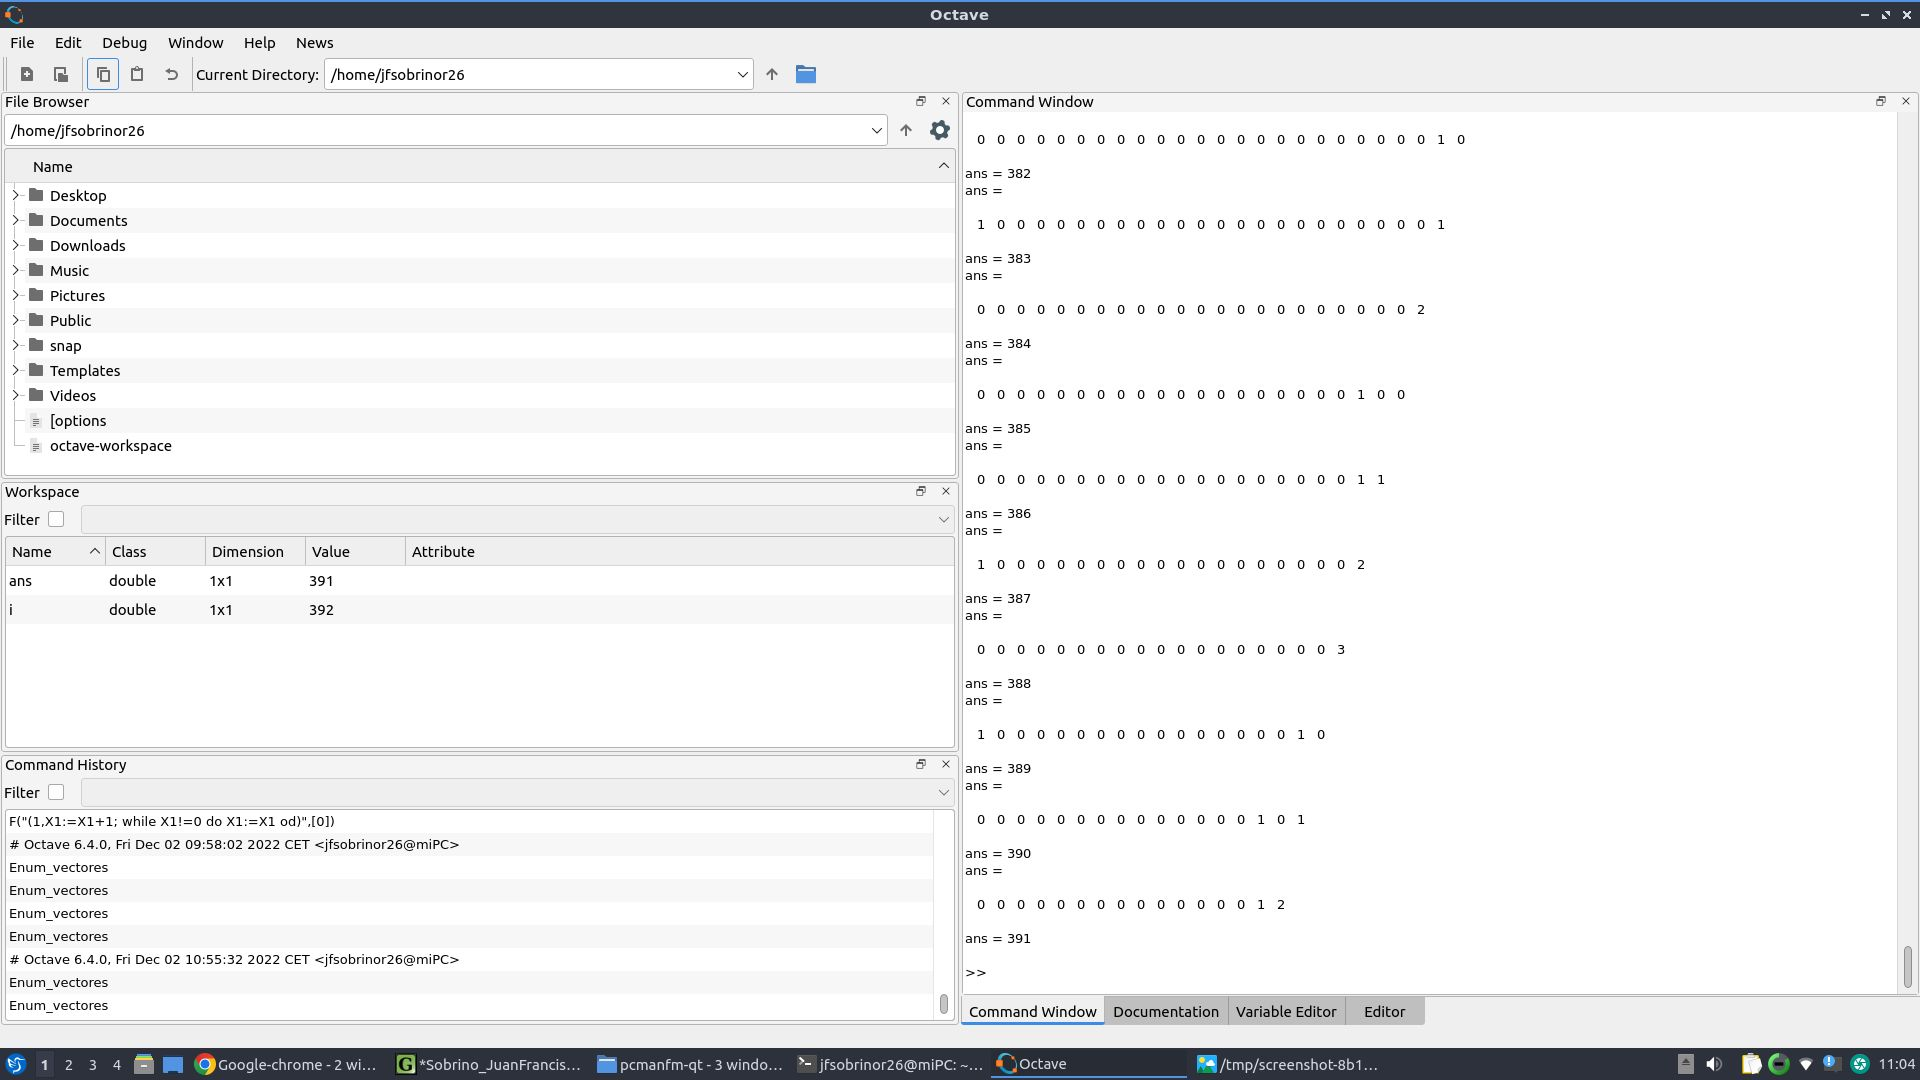
\includegraphics[scale=0.5]{EnumVectores.jpg}


\subsection*{
3.Create an Octave script that enumerates all the WHILE programs.
}
\begin{verbatim}
i=0
while(true)
    N2WHILE(i)
    i++
endwhile
\end{verbatim}

A continuación se muestra la enumeración de algunos programas WHILE:

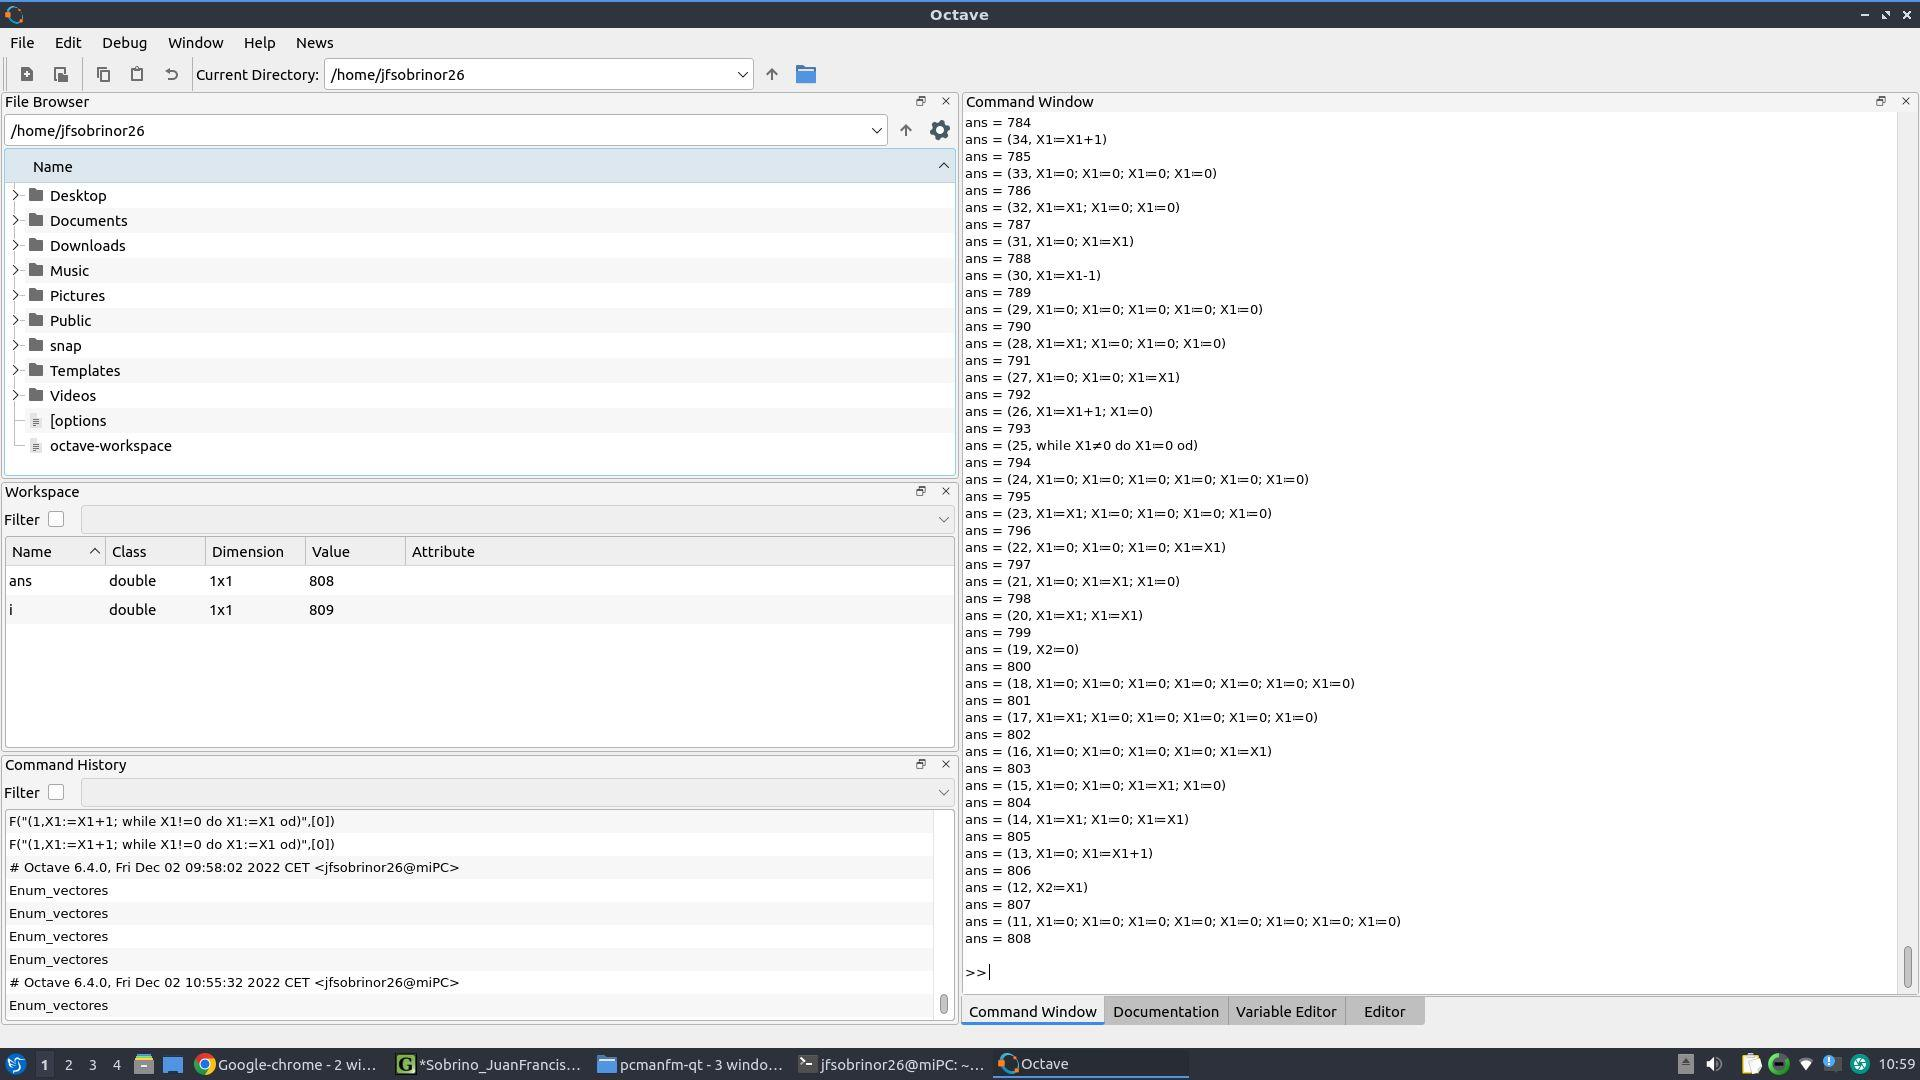
\includegraphics[scale=0.5]{Enum_WHILE-programs}

\end{document}